
\documentclass{article}
\usepackage{graphicx}
\graphicspath{ {Assignment2Files/} }
\usepackage{color}

\usepackage{amsmath}
\usepackage{amssymb}
\usepackage{listings}
\usepackage{algorithm2e}
\usepackage{float}

\usepackage{hyperref}
\hypersetup{linktoc=all}

\usepackage{listings}
\usepackage{geometry}
\geometry{margin=1in}
\usepackage{color}
\definecolor{light-gray}{gray}{0.95}
\lstset{numbers=right, 
                numberstyle=\tiny, 
                breaklines=true,
                backgroundcolor=\color{light-gray},
                numbersep=5pt,
                xleftmargin=.5in,
                xrightmargin=.5in} 

\sloppy
\definecolor{lightgray}{gray}{0.5}
\setlength{\parindent}{0pt}

\begin{document}

\title{Lab 2: JPEG Compression}
\author{Brian Hosler \& Sarah Peachey }
\maketitle 

\abstract{}
\tableofcontents
\newpage

\section{JPEG Quality Factor}

\qquad Peak Signal to Noise Ratio (PSNR) is a common method for measuring
the quality of a image that has gone through compression. PSNR is a way to
quanitize the quality of a decoded image as perceived by the human eye.
\eqref{psnr:1} is how PSNR is calculated, where $\sigma_e^2$ is the variance
of noise/error and A is the bit depth of the image. The value calculated can
be interpretted as unnoticable noise if it is greater than 40dB, as low
quality if it is less than 30dB, and as good quality otherwise. 

\begin{align}
	PSNR=10log_{10}(\frac{A^2}{\sigma_e^2})\label{psnr:1}
\end{align} 


\begin{lstlisting}[language=Matlab]
pep=imread('peppers.tif');
bab=imread('baboon.tif');

imwrite(pep, 'pep90.jpg','Quality',90)
imwrite(pep, 'pep70.jpg','Quality',70)
imwrite(pep, 'pep50.jpg','Quality',50)
imwrite(pep, 'pep30.jpg','Quality',30)
imwrite(pep, 'pep10.jpg','Quality',10)

imwrite(bab, 'bab90.jpg','Quality',90)
imwrite(bab, 'bab70.jpg','Quality',70)
imwrite(bab, 'bab50.jpg','Quality',50)
imwrite(bab, 'bab30.jpg','Quality',30)
imwrite(bab, 'bab10.jpg','Quality',10)

pep_psnr=zeros(1,6);
pep_size=zeros(1,6);

temp=imfinfo('peppers.tif');
pep_size(1)=temp.FileSize;
pep_psnr(1)= psnr(pep, pep);

temp=imfinfo('pep90.jpg');
pep_size(2)=temp.FileSize;
pep_psnr(2)= psnr(imread('pep90.jpg'), pep);

temp=imfinfo('pep70.jpg');
pep_size(3)=temp.FileSize;
pep_psnr(3)= psnr(imread('pep70.jpg'), pep);

temp=imfinfo('pep50.jpg');
pep_size(4)=temp.FileSize;
pep_psnr(4)= psnr(imread('pep50.jpg'), pep);

temp=imfinfo('pep30.jpg');
pep_size(5)=temp.FileSize;
pep_psnr(5)= psnr(imread('pep30.jpg'), pep);

temp=imfinfo('pep10.jpg');
pep_size(6)=temp.FileSize;
pep_psnr(6)= psnr(imread('pep10.jpg'), pep);

figure
subplot(2,1,1)
plot(100*[1 .9 .7 .5 .3 .1],pep_size,'--o')
hold on
title('peppers - file size vs quality')
subplot(2,1,2)
plot(100*[1 .9 .7 .5 .3 .1],pep_psnr,'--o')
hold on
title('peppers - psnr vs quality')

bab_psnr=zeros(1,6);
bab_size=zeros(1,6);

temp=imfinfo('baboon.tif');
bab_size(1)=temp.FileSize;
bab_psnr(1)= psnr(bab, bab);

temp=imfinfo('bab90.jpg');
bab_size(2)=temp.FileSize;
bab_psnr(2)= psnr(imread('bab90.jpg'), bab);

temp=imfinfo('bab70.jpg');
bab_size(3)=temp.FileSize;
bab_psnr(3)= psnr(imread('bab70.jpg'), bab);

temp=imfinfo('bab50.jpg');
bab_size(4)=temp.FileSize;
bab_psnr(4)= psnr(imread('bab50.jpg'), bab);

temp=imfinfo('bab30.jpg');
bab_size(5)=temp.FileSize;
bab_psnr(5)= psnr(imread('bab30.jpg'), bab);

temp=imfinfo('bab10.jpg');
bab_size(6)=temp.FileSize;
bab_psnr(6)= psnr(imread('bab10.jpg'), bab);

figure
subplot(2,1,1)
plot(100*[1 .9 .7 .5 .3 .1],bab_size,'--o')
hold on
title('baboon - file size vs quality')
subplot(2,1,2)
plot(100*[1 .9 .7 .5 .3 .1],bab_psnr,'--o')
hold on
title('baboon - psnr vs quality')
\end{lstlisting}

\newpage
In the following table the peppers.tif and baboon.tif were compressed with
image quality factors of 90, 70, 50, 30, \& 10. 

\begin{center}
\hspace*{-2.5cm}
\begin{tabular}{@{}c|c|c}
\textbf{Quality Factor} & \textbf{Peppers} & \textbf{Baboon} \\  
\hline
\textbf{90} & 
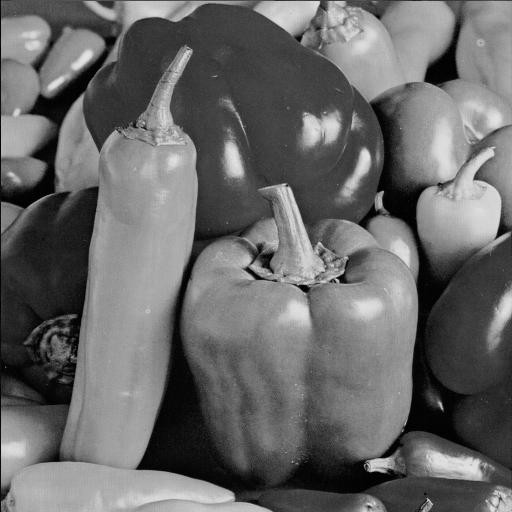
\includegraphics[width=0.4\textwidth]{pep90}
&
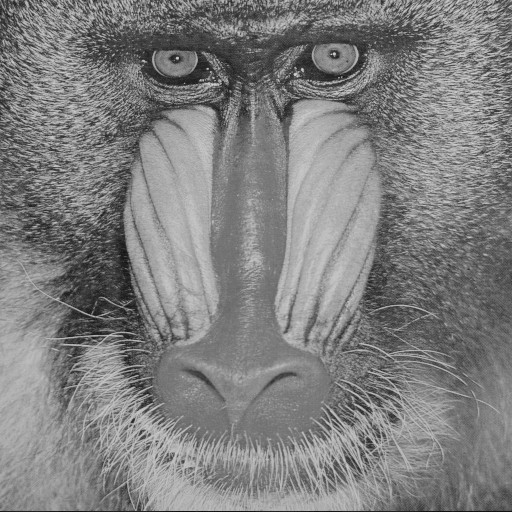
\includegraphics[width=0.4\textwidth]{bab90}
\\ \hline
\textbf{70} & 
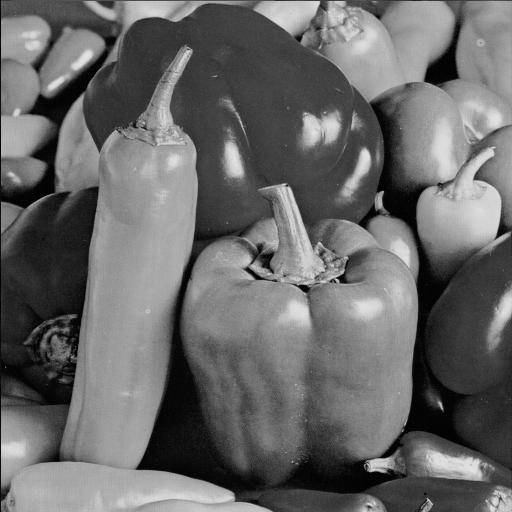
\includegraphics[width=0.4\textwidth]{pep70}
&
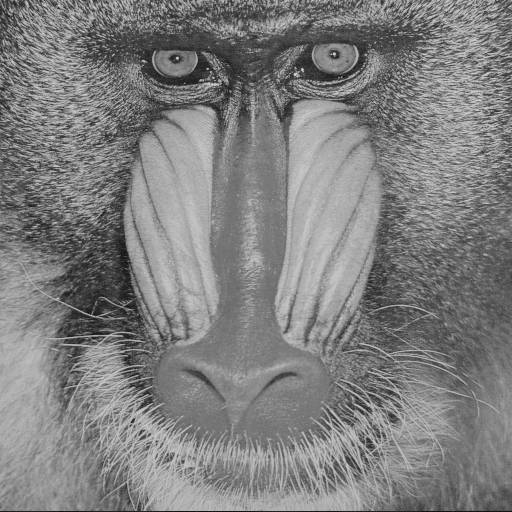
\includegraphics[width=0.4\textwidth]{bab70}
\\ \hline
\textbf{50} & 
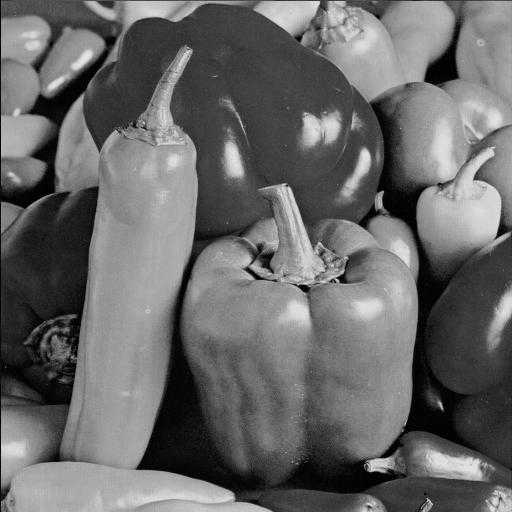
\includegraphics[width=0.4\textwidth]{pep50}
&
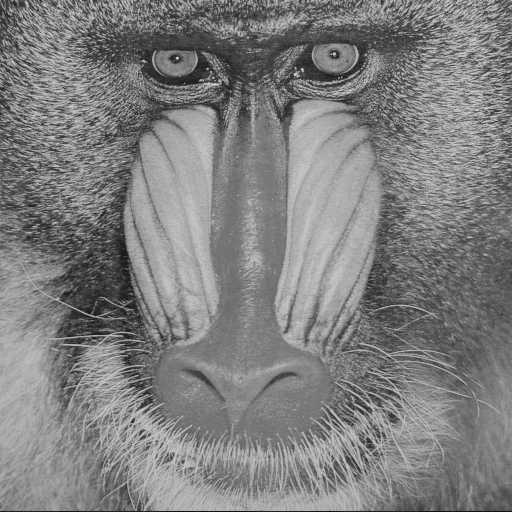
\includegraphics[width=0.4\textwidth]{bab50}
\\ \hline
\end{tabular}
\hspace*{-2.5cm}
\end{center}
\begin{center}
\hspace*{-2.5cm}
\begin{tabular}{@{}ccc}
\textbf{30} & 
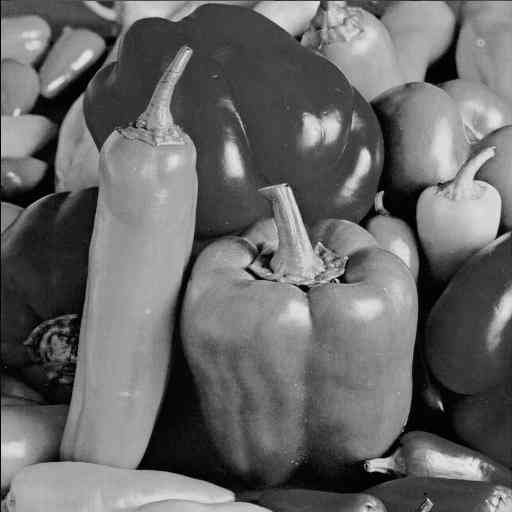
\includegraphics[width=0.4\textwidth]{pep30}
&
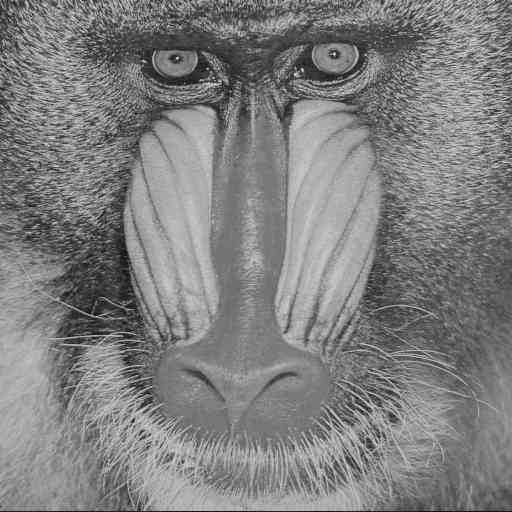
\includegraphics[width=0.4\textwidth]{bab30}
\\ \hline
\textbf{10} & 
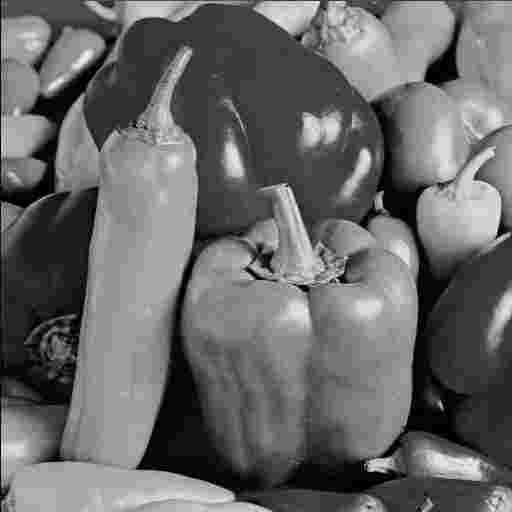
\includegraphics[width=0.4\textwidth]{pep10}
&
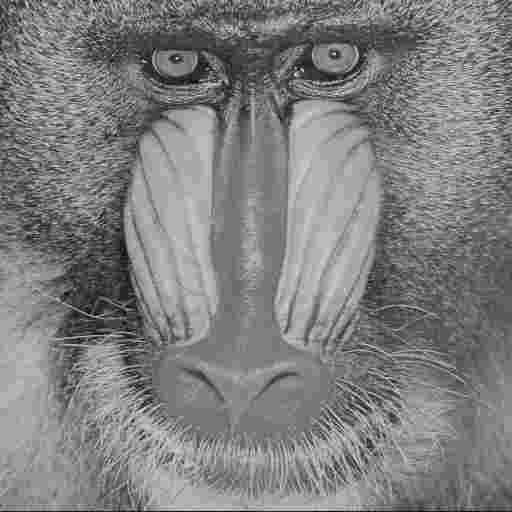
\includegraphics[width=0.4\textwidth]{bab10}
\\
\end{tabular}
\hspace*{-2.5cm}
\end{center}

\hfill \break 

As seen in figures \ref{pepperGraph}, and \ref{baboonGraph} as the image
file size gets smaller the PSNR of the image drops lower. Also, as seen in
the images as the quality gets lower the image becomes more blocky and noise
in added in the high freqency sections. Which is normally fine because the
human eye is less perceptive to changes in high frequency regions, but edge
also count as high frequency and noise can be perceived on edged of smooth
regions. 
The blockiness occurs because jpeg divides the image into $8 \ x \ 8$ block
and then runs the algorithm on each block, therefore, some block may throw away or
keep more information than the one next to it. Also the jpeg algorithm takes
into account the humans do not perceive change in high frequency regions as
well, so it will discrad this information. 

There is a clear drop in image quality around a quality factor of 30 or 10.
The image becomes far more blocky because of the loss in information. The
PSNR graphs also reflect this, because the peppers at quality 10 have a PSNR
of about 30, and the baboon at quality of 30 drops below 30dB. Since less
than 30dB is the qualification for low quality it make sense that these
images have visually perceived error.

\begin{figure}[H]
\centering
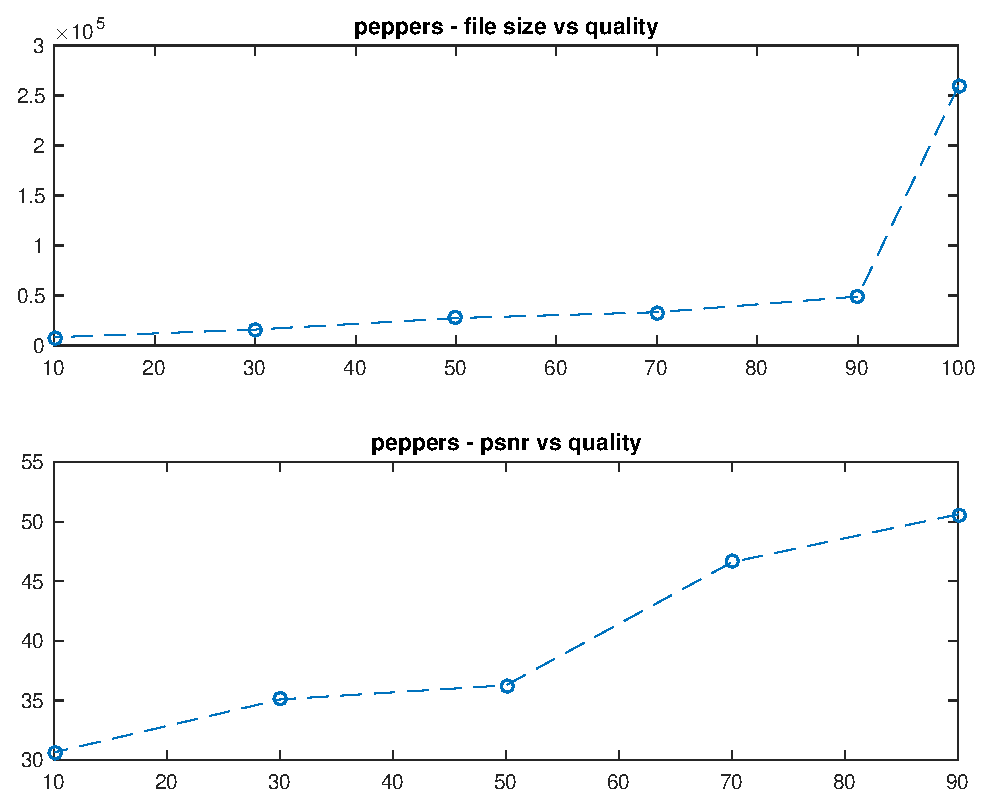
\includegraphics [width=4in]{lab2_01.eps}
\caption{Peppers file size and PSNR as the quality changes}
\label{pepperGraph}
\end{figure}

\begin{figure}[H]
\centering
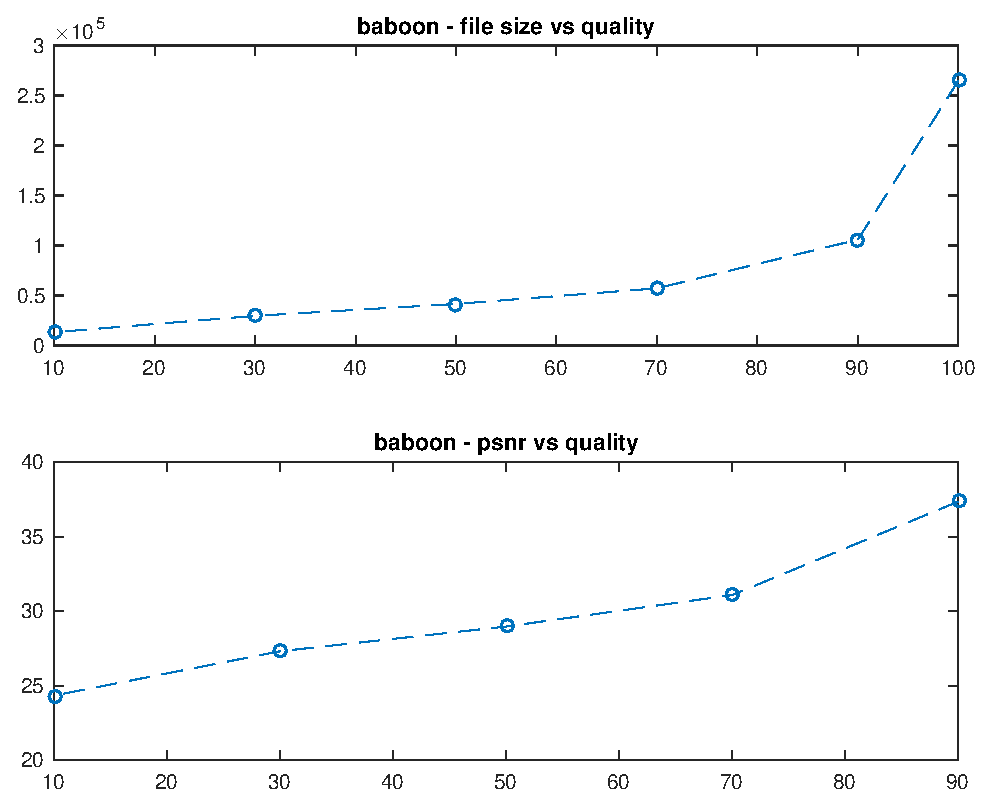
\includegraphics [width=4in]{lab2_02.eps}
\caption{Baboon file size and PSNR as the quality changes}
\label{baboonGraph}
\end{figure}

\newpage
\section{Writing JPEG compression in matlab}

\qquad The following sections are the code the implements the jpeg encoding
algorithm by segmenting the image into $8 \ x \ 8$ pixel blocks, computing
the discrete cosine tranform, and quanitizing each block. Then using the
provided functions to further format and entropy encode the jpeg. That
process is then reversed for decoding the image. 

\subsection*{myJpgEncode.m}
\begin{lstlisting}[language=Matlab]
function [result] = myJpgEncode( pep,Q )
%myJpgEncode implement my own jpeg algorithm
%   using the notes 
A=zeros(size(pep)); 
stor=[];
for i=1:512/8
    for j=1:512/8
        tempA=dct2(pep(8*(i-1)+1:i*8,8*(j-1)+1:j*8)); 
        pep_quan=round(tempA./Q).*Q; 
        stor=[stor;ZigzagMtx2Vector(pep_quan)];
    end 
end
result=JPEG_entropy_encode(512,512,8,Q,stor,'./',1);
end
\end{lstlisting}


\subsection*{myJpgDecode.m}
\begin{lstlisting}[language=Matlab]
function [pep] = myJpgDecode()
%myJpgEncode implement my own jpeg algorithm
%   using the notes 
[rowN,colN,dct_block_size,iQ,iZZDCTQIm]=JPEG_entropy_decode('./');
pep=zeros(512);
ndx=1;
for i=1:512/8
    for j=1:512/8
        pep(8*(i-1)+1:i*8,8*(j-1)+1:j*8)=idct2(Vector2ZigzagMtx(iZZDCTQIm(ndx,:)));
        ndx=ndx+1;
    end 
end 
end
\end{lstlisting}


\newpage
\section{Evaluating Quantization Tables}
\qquad Our jpeg encoding and decoding algorithms are then tested by using
the standard jpeg luminance quantization table. Then a custom quantization
table is created based off of the values from the DCT of the peppers.tif
image. This custom table should better compress the image, without loosing
too much information as to distort the image.  

\begin{lstlisting}[language=Matlab]
Q=[16 11 10 16 24 40 51 61;...
   12 12 14 19 26 58 60 55;...
   14 13 16 24 40 57 69 56;...
   14 17 22 29 51 87 80 62;...
   18 22 37 56 68 109 103 77;...
   24 35 55 64 81 104 113 92;...
   49 64 78 87 103 121 120 101;...
   72 92 95 98 112 100 103 99];

tempQ=zeros(8);
for i=1:512/8
    for j=1:512/8
        tempQ=tempQ+abs(dct2(pep(8*(i-1)+1:i*8,8*(j-1)+1:j*8)));
    end
end
DCTs=tempQ/4096;
nrm1=max(max(DCTs))./DCTs;
Q2=double(uint8(nrm1.^.65));

stor=[];
for i=1:512/8
    for j=1:512/8
        tempA=dct2(pep(8*(i-1)+1:i*8,8*(j-1)+1:j*8));
        stor=[stor;ZigzagMtx2Vector(tempA)];
    end
end
vrnce=Vector2ZigzagMtx(var(stor));
nrm2=max(max(vrnce))./vrnce;
Q3=double(uint8(log(nrm2).^2))+1;

A=myJpgEncode( pep,Q );
jpg1=uint8(myJpgDecode());
psnr(pep,jpg1)

B=myJpgEncode( pep,Q2 );
jpg2=uint8(myJpgDecode());
psnr(pep,jpg2)

C=myJpgEncode( pep,Q3 );
jpg3=uint8(myJpgDecode());
psnr(pep,jpg3)

figure
imshow([pep,jpg1;jpg2,jpg3])
\end{lstlisting}

** NOTE: Put some words about the actual Quantization tables used and the
results of each one, in terms of PSNR and visual perception. **


\begin{table}[H]
\centering
\begin{tabular}{ |c|c|c| } 
 \hline
 Q-Table & Compressed Size(kB) & PSNR(dB) \\ 
 \hline
 Standard 	& 44.7 & 36.27 \\ 
 Mean 		& 33.1 & 36.33 \\ 
 Variance 	& 23.7 & 34.40 \\ 
 \hline
\end{tabular}
\caption{Comparison of Different JPEG Quantization Tables Used}
\label{snrTab}
\end{table}
   
\begin{figure}[H]
\centering
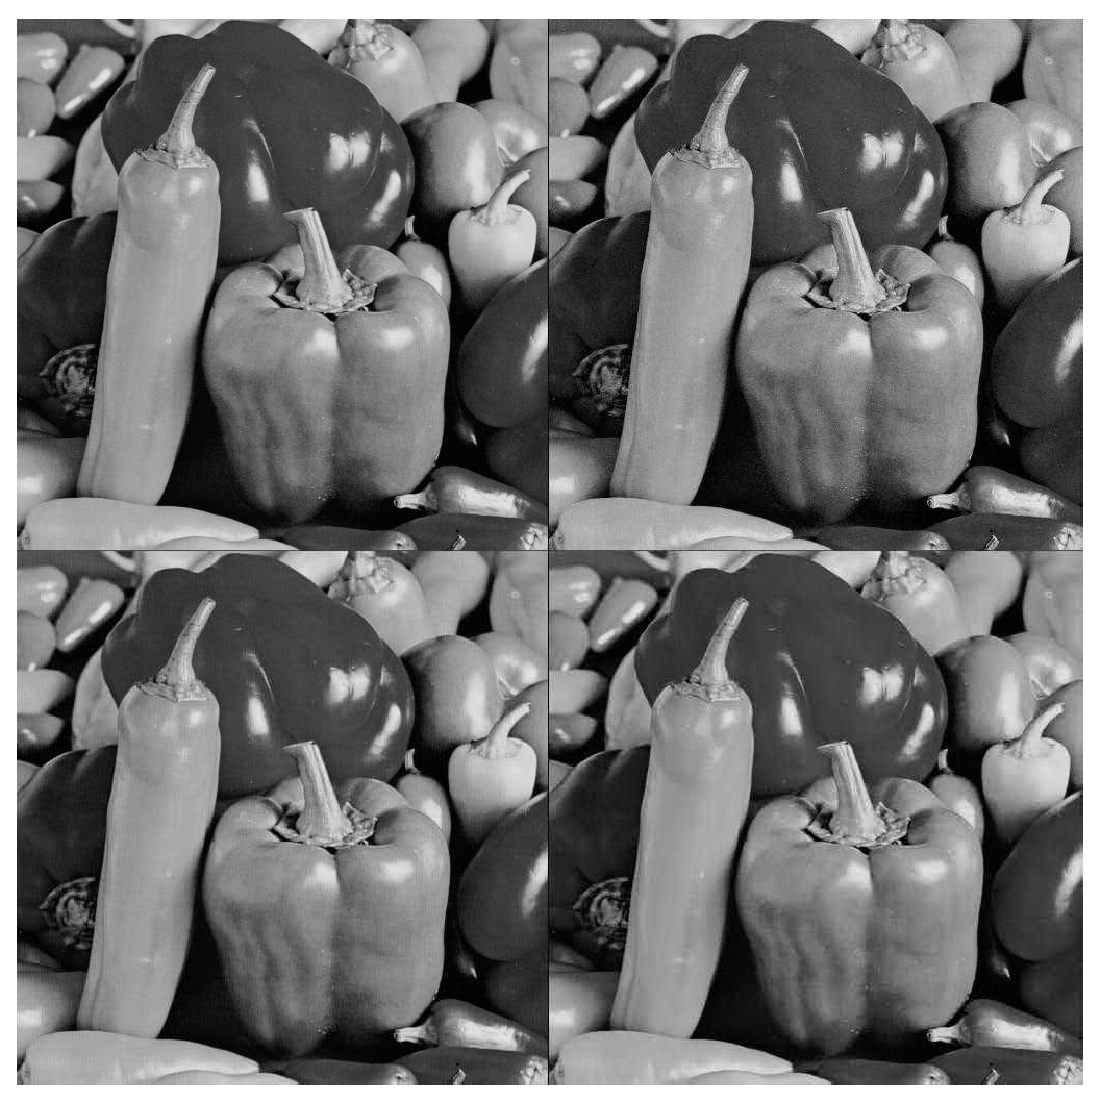
\includegraphics [width=4in]{lab2_03.eps}
\caption{Resultant image after no JPEG compression(top-left),
compression using the JPEG standard quantization table(top-right),
compression using a quantization table based on the mean magnitude of the DCT coefficients(bottom-left), and
compression using a quantization table derived from the DCT coefficients' variences(bottom-right).}
\label{jpgTables}
\end{figure}


\end{document}
    
